\section{Metrics of 6 networks}
In this section I will present some statistics about the 6 chosen networks. The results will be presented in tables. All metrics and plots were calculated and generated using the Python package NetworkX.

\begin{table}
    \centering
    \begin{tabular}{|p{0.19\linewidth}|c|c|c|c|c|c|c|}
        \hline
        \textbf{Metric} & \textbf{Net. 1} & \textbf{Net. 2} & \textbf{Net. 3} & \textbf{Net. 4} & \textbf{Net. 5} & \textbf{Net. 7} \\
        \hline
        Num. Nodes & 60 & 60 & 59 & 60 & 59 & 60 \\
        \hline
        Num. Edges & 426 & 120 & 73 & 48 & 30 & 214 \\
        \hline
        Density & 0.120 & 0.067 & 0.042 & 0.027 & 0.017 & 0.120 \\
        \hline
        Avg. Clust. Coef. & 0.394 & 0.304 & 0.296 & 0.241 & 0.168 & 0.488 \\
        \hline
        Num. Nodes SCC & 49 & - & - & - & - & - \\
        \hline
        Num. Nodes WCC & 58 & - & - & - & - & - \\
        \hline
        Num. Nodes CC & - & 52 & 42 & 20 & 10 & 59 \\
        \hline
        Avg. Path Len. SCC & 2.599 & - & - & - & - & - \\
        \hline
        Avg. Path Len. CC & - & 3.143 & 4.234 & 2.857 & 1.711 & 2.654 \\
        \hline
        Diameter of SCC & 7 & - & - & - & - & - \\
        \hline
        Diameter of CC & - & 7 & 11 & 6 & 4 & 6 \\
        \hline
    \end{tabular}
    \caption{Network statistics}
    \label{table:1}
\end{table}

\subsection{Number of nodes}
The number of nodes of each graph is the amount of people who have participated in the survey. Whether they are connected to someone else, or not, they will be represented as nodes.

\subsection{Number of edges}
The number of edges of each graph will be the amount of connections that exist between each person for each question.

\subsection{Edge density}
Graph density tells us how connected nodes are between each other. If the density value is high, we say the graph is connected, if the density value is low, we say it is sparse. For undirected graphs, this metric can be calculated as
\begin{equation}
    D_{undirected} = \frac{2|E|}{|N|(|N|-1)}
    \label{equation:dir_density}
\end{equation}
and the density for directed graphs is defined as
\begin{equation}
    D_{directed} = \frac{|E|}{|N|(|N    |-1)}
    \label{equation:undir_density}
\end{equation}
where $E$ is the number of edges and $V$ is the number of nodes in the graph.

\subsection{Degree distribution}
The degree distribution can superficially tell us what are the preferences for people when connecting to each other. Figure \ref{fig:4} plots the degree distributions for the 6 chosen networks.
\begin{figure}
    \centering
    \subfloat[\centering Network 1]{{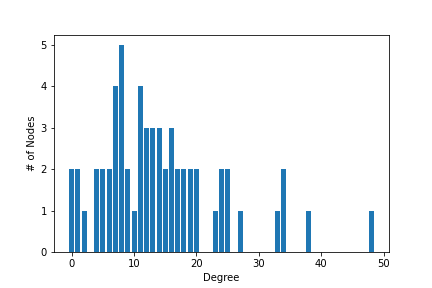
\includegraphics[width=0.45\textwidth]{img/net_0_degree_distribution.png}}}
    \qquad
    \subfloat[\centering Network 2]{{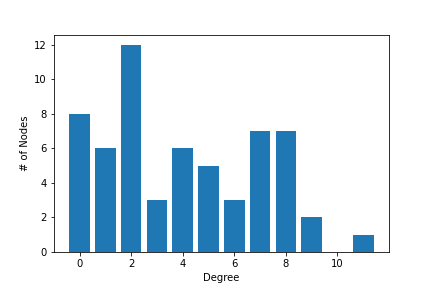
\includegraphics[width=0.45\textwidth]{img/net_1_degree_distribution.png}}}
    \qquad
    \subfloat[\centering Network 3]{{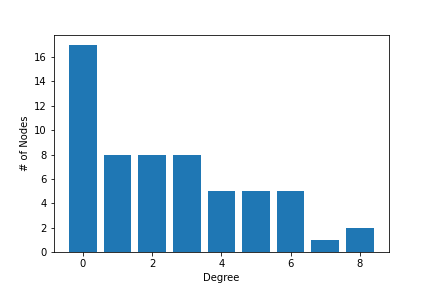
\includegraphics[width=0.45\textwidth]{img/net_2_degree_distribution.png}}}
    \qquad
    \subfloat[\centering Network 4]{{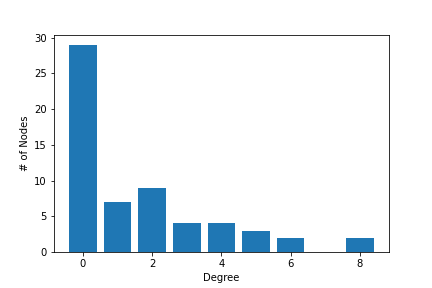
\includegraphics[width=0.45\textwidth]{img/net_3_degree_distribution.png}}}
    \qquad
    \subfloat[\centering Network 5]{{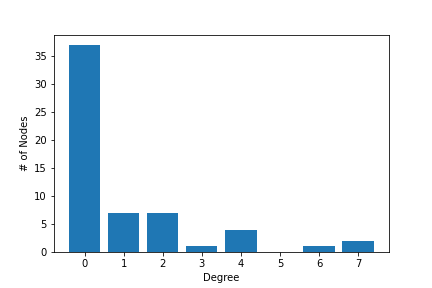
\includegraphics[width=0.45\textwidth]{img/net_4_degree_distribution.png}}}
    \qquad
    \subfloat[\centering Network 7]{{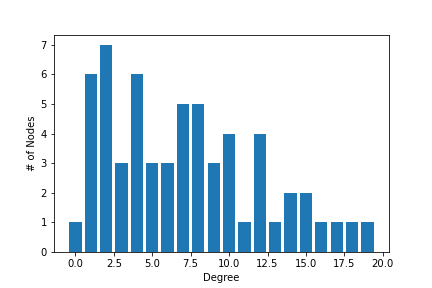
\includegraphics[width=0.45\textwidth]{img/net_6_degree_distribution.png}}}
    \caption{Degree distributions}
    \label{fig:4}
\end{figure}

\subsection{Average clustering coefficient}
The average clustering coefficient for a graph helps determine how transitive a relationship is. For example, if persons A and B are friends, and persons A and C are friends, there is a high chance that persons B and C are also friends. The clustering coefficient is defined as
\begin{equation}
    C_i = \frac{2e_i}{k_i(k_i-1)}
    \label{equation:clustering_coef}
\end{equation}
where $e_i$ is the number of edges between the neighbors of node $i$.

The average clustering coefficient of the graph is calculated as
\begin{equation}
    \left\langle C \right\rangle = \frac{1}{N}\sum_{i}^{N}C_i
    \label{equation:avg_clustering_coef}
\end{equation}
where $N$ is the number of nodes in the graph, and $C_i$ is the clustering coefficient of node $i$.

\subsection{Number of nodes in strongly connected component (SCC)}
The strongly connected component (SCC) metric can only be obtained from directed graphs. Since only the first network is directed, it is the only one that can provide this value. For networks 2 through 5, and 7, the values are from the connected components. Refer to table \ref{table:1} for the values.

\subsection{Number of nodes in weakly connected component (WCC)}
The weakly connected component (WCC) metric can only be obtained from directed graphs. Since only the first network is directed, it is the only one that can provide this value. For networks 2 through 5, and 7, the values are from the connected components. Refer to table \ref{table:1} for the values.

\subsection{Average path length in SCC}
The average path length metric indicates how far apart two nodes are from each other in the connected graph. In other words, how many jumps, in average, it takes to reach other nodes. For a directed graph, it is calculated as
\begin{equation}
    \left\langle d \right\rangle \equiv \frac{1}{2L_{max}}\sum_{i,j \neq i}d_{ij}
    \label{equation:dir_avg_path_len}
\end{equation}
whereas for undirected graphs, it is calculated as
\begin{equation}
    \left\langle d \right\rangle \equiv \frac{1}{L_{max}}\sum_{i,j >  i}d_{ij}
    \label{equation:undir_avg_path_len}
\end{equation}

For networks 2 through 5, and 7, I calculated the average path length in the connected component because these networks are undirected graphs, thus not being possible to determine strongly connected components.

\subsection{Diameter of SCC}
This metric represents the maximum shortest distance between two nodes in a connected graph. It is be represented as
\begin{equation}
    diameter \equiv \max_{ij}d_{ij}
    \label{equation:diameter}
\end{equation}

For the first network, I collected the diameter of the strongly connected component. However, since all other networks are undirected graphs, I collected the diameter of the largest connected component.

\subsection{Community detection}
To detect communities in each of the chosen networks, I ran the Girvan--Newman algorithm, implemented in NetworkX. Figure \ref{fig:5} illustrates the communities in each network. The communities the algorithm found make sense, given that it ran by removing the edges with highest betweenness, separating the communities the edge held together. Also, by comparing with figures \ref{fig:1}, \ref{fig:2}, and \ref{fig:3}, we can see that the nodes with most connections between each other form a community the algorithm was able to find. Another interesting feature that the community detection algorithm allows us to perceive is that the more sparse the graph, the more communities we have. Figures \ref{fig:comm_3}, \ref{fig:comm_4}, and \ref{fig:comm_5} depict this behavior.
\begin{figure}[t]
    \centering
    \subfloat[\centering Network 1]{{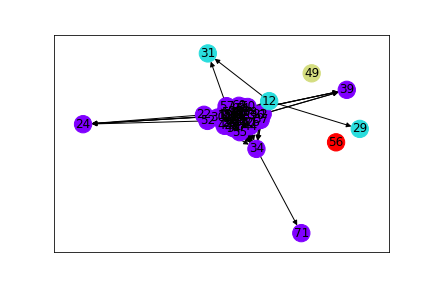
\includegraphics[width=0.45\textwidth]{img/net_0_communities.png}\label{fig:comm_1}}}
    \qquad
    \subfloat[\centering Network 2]{{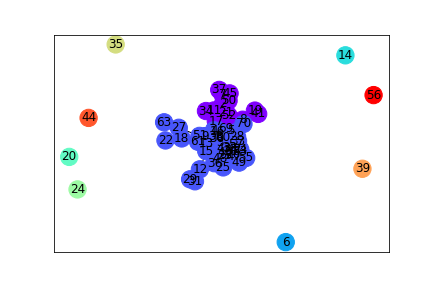
\includegraphics[width=0.45\textwidth]{img/net_1_communities.png}\label{fig:comm_2}}}
    \qquad
    \subfloat[\centering Network 3]{{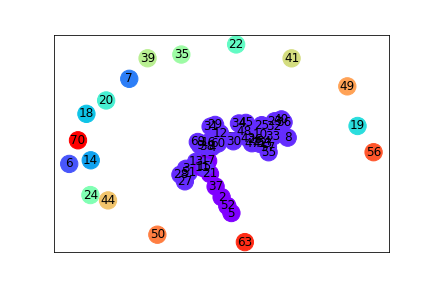
\includegraphics[width=0.45\textwidth]{img/net_2_communities.png}\label{fig:comm_3}}}
    \qquad
    \subfloat[\centering Network 4]{{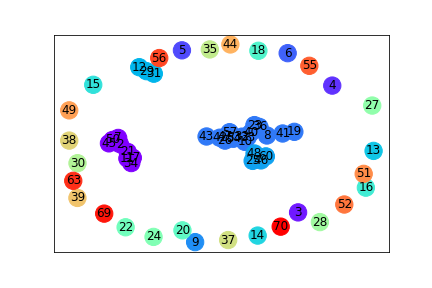
\includegraphics[width=0.45\textwidth]{img/net_3_communities.png}\label{fig:comm_4}}}
    \qquad
    \subfloat[\centering Network 5]{{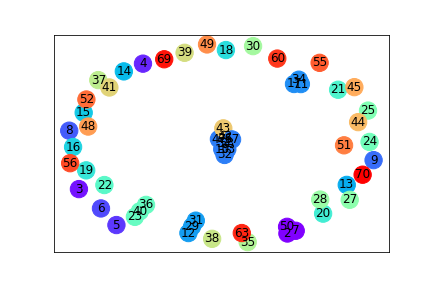
\includegraphics[width=0.45\textwidth]{img/net_4_communities.png}
    \label{fig:comm_5}}}
    \qquad
    \subfloat[\centering Network 7]{{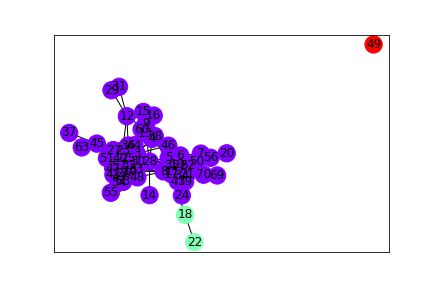
\includegraphics[width=0.45\textwidth]{img/net_6_communities.png}
    \label{fig:comm_7}}}
    \caption{Detected Communities}
    \label{fig:5}
\end{figure}

\subsection{Centrality Measures}
Centrality tries to determine which node is the most central in a graph. The four centrality measures will be used to determine which node is the most important in each network. The measures are in-degree, out-degree, betweenness, and closeness. The choice for each centrality measure for each graph was arbitrary.

\subsubsection{Network 1}
For this network, in-degree and out-degree will be used to determine the two most central nodes. Because it is a directed graph, we can use these measures. The in-degree centrality of a node is calculated based on how many edges arrive in it. Similarly, the out-degree centrality of a node is calculated based on how many edges leave it. Table \ref{table:2} summarizes the two most people.
\begin{table}
    \centering
    \subfloat[\centering In-degree]{{
        \begin{tabular}{|c|c|c|}
            \hline
            \textbf{Rank} & \textbf{Person} & \textbf{Score} \\
            \hline
            1 & 17 & 0.576 \\
            \hline
            2 & 5 & 0.508 \\
            \hline
        \end{tabular}
        \label{table:net_0_in_deg}
    }}
    \qquad
    \subfloat[\centering Out-degree]{{
        \begin{tabular}{|c|c|c|}
            \hline
            \textbf{Rank} & \textbf{Person} & \textbf{Score} \\
            \hline
            1 & 10 & 0.271 \\
            \hline
            2 & 19 & 0.254 \\
            \hline
        \end{tabular}
        \label{table:net_0_out_deg}
    }}
    \caption{Network 1 centrality}
    \label{table:2}
\end{table}

\subsubsection{Network 2}
The centrality measures analyzed for this network were degree centrality and betweenness centrality. Degree centrality is similar to in-degree and out-degree centrality measures, except for the direction of the edges, which do not exist. The degree centrality measure for a node is defined by the amount of edges connected to it. Betweenness, on the other hand, is defined by the amount of shortest paths that go through a given node, and is calculated as follows
\begin{equation}
    C_B(i) = \sum_{j<k}\frac{g_{jk}(i)}{g_{jk}}
    \label{equation:betweenness_centrality}
\end{equation}
where $g_{jk}$ is the amount of shortest paths connecting nodes $j$ and $k$, and $g_{jk}(i)$ is the node currently being analyzed. Table \ref{table:3} summarizes the values found.
\begin{table}
    \centering
    \subfloat[\centering Degree]{{
        \begin{tabular}{|c|c|c|}
            \hline
            \textbf{Rank} & \textbf{Person} & \textbf{Score} \\
            \hline
            1 & 10 & 0.186 \\
            \hline
            2 & 42 & 0.152 \\
            \hline
        \end{tabular}
        \label{table:net_1_deg}
    }}
    \qquad
    \subfloat[\centering Betweenness]{{
        \begin{tabular}{|c|c|c|}
            \hline
            \textbf{Rank} & \textbf{Person} & \textbf{Score} \\
            \hline
            1 & 17 & 0.169 \\
            \hline
            2 & 30 & 0.131 \\
            \hline
        \end{tabular}
        \label{table:net_1_bet}
    }}
    \caption{Network 2 centrality}
    \label{table:3}
\end{table}

\subsubsection{Network 3}
The chosen centrality measures for this network were degree and closeness. Degree centrality has been previously defined. However, the closeness centrality measure is defined by the average length of shortest paths between a node and all other nodes in a graph. It can be calculated as
\begin{equation}
    C_C(i) = \left[\frac{1}{N-1}\sum_{j=1}^{N}d(i,j)\right]^{-1}
\end{equation}
where $N$ is the number of nodes in a graph, and $d(i,j)$ is the distance between nodes $i$ and $j$. Table \ref{table:4} summarizes the centrality results for this network.
\begin{table}
    \centering
    \subfloat[\centering Degree]{{
        \begin{tabular}{|c|c|c|}
            \hline
            \textbf{Rank} & \textbf{Person} & \textbf{Score} \\
            \hline
            1 & 48 & 0.137 \\
            \hline
            2 & 42 & 0.137 \\
            \hline
        \end{tabular}
        \label{table:net_2_deg}
    }}
    \qquad
    \subfloat[\centering Closeness]{{
        \begin{tabular}{|c|c|c|}
            \hline
            \textbf{Rank} & \textbf{Person} & \textbf{Score} \\
            \hline
            1 & 48 & 0.245 \\
            \hline
            2 & 30 & 0.243 \\
            \hline
        \end{tabular}
        \label{table:net_2_bet}
    }}
    \caption{Network 3 centrality}
    \label{table:4}
\end{table}

\subsubsection{Network 4}
The centrality measures chosen to analyze from this network were betweenness and closeness. These two measures have been previously defined. Table \ref{table:5} summarizes the values found.
\begin{table}
    \centering
    \subfloat[\centering Betweenness]{{
        \begin{tabular}{|c|c|c|}
            \hline
            \textbf{Rank} & \textbf{Person} & \textbf{Score} \\
            \hline
            1 & 10 & 0.039 \\
            \hline
            2 & 33 & 0.032 \\
            \hline
        \end{tabular}
        \label{table:net_3_bet}
    }}
    \qquad
    \subfloat[\centering Closeness]{{
        \begin{tabular}{|c|c|c|}
            \hline
            \textbf{Rank} & \textbf{Person} & \textbf{Score} \\
            \hline
            1 & 10 & 0.169 \\
            \hline
            2 & 33 & 0.165 \\
            \hline
        \end{tabular}
        \label{table:net_3_close}
    }}
    \caption{Network 4 centrality}
    \label{table:5}
\end{table}

\subsubsection{Network 5}
The centrality measures analyzed for this network were degree and betweenness centralities. These measures already have been introduced. Table \ref{table:6} summarizes the two most influential nodes of this network and their centrality score.
\begin{table}
    \centering
    \subfloat[\centering Degree]{{
        \begin{tabular}{|c|c|c|}
            \hline
            \textbf{Rank} & \textbf{Person} & \textbf{Score} \\
            \hline
            1 & 53 & 0.120 \\
            \hline
            2 & 54 & 0.120 \\
            \hline
        \end{tabular}
        \label{table:net_4_deg}
    }}
    \qquad
    \subfloat[\centering Betweenness]{{
        \begin{tabular}{|c|c|c|}
            \hline
            \textbf{Rank} & \textbf{Person} & \textbf{Score} \\
            \hline
            1 & 42 & 0.005 \\
            \hline
            2 & 53 & 0.004 \\
            \hline
        \end{tabular}
        \label{table:net_4_bet}
    }}
    \caption{Network 5 centrality}
    \label{table:6}
\end{table}

\subsubsection{Network 7}
The chosen centrality measures for network 7 were degree and closeness. I will refrain from going deeper into these concepts since they have already been introduced. Table \ref{table:7} summarizes the centrality findings for this network.
\begin{table}
    \centering
    \subfloat[\centering Degree]{{
        \begin{tabular}{|c|c|c|}
            \hline
            \textbf{Rank} & \textbf{Person} & \textbf{Score} \\
            \hline
            1 & 3 & 0.322 \\
            \hline
            2 & 28 & 0.305 \\
            \hline
        \end{tabular}
        \label{table:net_6_deg}
    }}
    \qquad
    \subfloat[\centering Closeness]{{
        \begin{tabular}{|c|c|c|}
            \hline
            \textbf{Rank} & \textbf{Person} & \textbf{Score} \\
            \hline
            1 & 28 & 0.543 \\
            \hline
            2 & 17 & 0.509 \\
            \hline
        \end{tabular}
        \label{table:net_6_close}
    }}
    \caption{Network 7 centrality}
    \label{table:7}
\end{table}
